% =============================================================
%   《经济与社会》课程论文
%   排版样式：PRL / REVTeX 4-2，中文用 ctex 包
%   编译建议：
%     xelatex paper.tex
%     xelatex paper.tex
% =============================================================
\documentclass[aps,prl,reprint,superscriptaddress,floatfix,nofootinbib,longbibliography,amsmath,amssymb]{revtex4-2}

% ---- 中文支持 (xelatex + ctex) ----
\usepackage[UTF8,fontset=fandol,scheme=plain]{ctex}

\usepackage{graphicx}
\usepackage{booktabs}
\usepackage{array}
\usepackage{bm}
\usepackage{xcolor}
\usepackage{hyperref}
\hypersetup{unicode=true,colorlinks=true,linkcolor=blue!50!black,
            citecolor=blue!50!black,urlcolor=blue!50!black}

\usepackage[font=small,labelfont=bf,labelsep=period]{caption}

\graphicspath{{figures/}{data/figures/}{output/figures/}}

\newcommand{\kms}{\ensuremath{\,\mathrm{km}}}
\newcommand{\marginvar}{\ensuremath{\mathrm{margin}}}
\newcommand{\DataPageUrl}{https://github.com/Tsuihan-sudo/economy-society-paper}
\newcommand{\RawPoiDataUrl}{https://github.com/Tsuihan-sudo/economy-society-paper/data/amap_poi_raw.csv}
\newcommand{\AuditDataUrl}{https://github.com/Tsuihan-sudo/economy-society-paper/data/poi_classification_audit.csv}

\begin{document}

\title{城市中心生产活动的集聚阈值与上海 POI 证据}

\author{杜宇航}
\email{22307110210@m.fudan.edu.cn}
\affiliation{复旦大学，物理学系}

\date{\today}

\begin{abstract}
城市中心通常被视为制造业的反面：地价高昂、交通拥堵、监管密集。本文给出一个有条件的结论：中心区排斥的主要是土地密集、物流密集和污染密集的传统制造；而接纳低污染、低土地强度、高知识密度且依赖快速迭代的城市型生产。我们将工厂留在城市中心与否视作收益与成本相互竞争的结果，其中收益来自集聚、知识和速度，成本来自地租、监管、物流和一般拥挤，并把这一机制编码为一个无量纲线性阈值模型，为不同行业类型赋予六维先验参数并作随机扰动检验。数值模拟显示，研发试制、样衣打版、数字内容生产和城市微工厂等典型活动位于城市中心可行性阈值线上方，而传统重型制造、仓储/粗加工和标准化装配则更适合外围。进一步采集高德地图平台上海生产活动兴趣点（Point of Interest, POI）数据构造一个描述性空间样本，算法规则保留 2756 条 POI，其中传统制造 1072 条、城市型生产 476 条。城市型生产到人民广场（上海城市核心区）的平均距离为 18.94 公里，传统制造为 28.16 公里；在多城市中心口径下，二者到最近中心/副中心的平均距离分别为 11.59 和 19.78 公里。本文不作因果性识别，而将其作为与理论机制一致的描述性证据：现代城市中心并非完全排斥生产，而是筛选生产类型；中心区保留的是知识密集、低负外部性且高协同需求的生产环节。
\end{abstract}

\maketitle

\section{引言}

城市中心能否存在工厂，不是一个单纯的是/否问题，在展开讨论之前应先定义明晰问题对象。若工厂指占地大、污染高、货车频繁进出的传统制造，中心区通常不是合适位置：土地机会成本高，物流压力大，监管力度严，传统制造很难与办公、居住、商业和公共空间竞争。若工厂被理解为更宽泛的生产活动，结论将不同。设计打样、研发试制、小批量定制、数字内容生产、中央厨房和园区平台仍处于某生产链条中，却未必需要大面积土地和重物流；它们更依赖设计研发、客户反馈、专业服务、面对面协同和高技能劳动力。

本文核心结论是：城市中心并非不能容纳工厂，而是更适合城市型生产。这里的``城市型生产''指低污染、低土地强度、高知识密度、高协同需求、高交付速度的生产环节。其与传统制造的差异，不在于是否``生产''，而在于中心区的集聚收益能否覆盖中心区的相对成本。这一判断直接来自课程中关于生产型城市、集聚外部性、竞租模型、城市规模成本和技术变迁的讨论\cite{lec2,lec4,lec5,lec7,lec8,lec10}。

本文将展示两组结果支撑这一结论。第一，通过构建一个简单的线性阈值模型，数值模拟显示，当集聚、知识和速度收益大于地租、监管、物流和一般拥挤成本时，生产活动可以留在中心。为避免模型被质疑为无意义的调参游戏，正文将列举行业六维参数并陈述赋值理由，更进一步用两类随机扰动检验核心排序是否依赖于精确赋值。第二，上海 POI 数据显示，城市型生产比传统制造更接近中心；这一事实在人民广场单中心口径和多中心口径下均成立。分析不作因果识别，也不把 POI 视为完整企业名录，但能够作为理论机制成立的事实性证据。

\section{阈值模型}

课程中对工厂镇的讨论说明，生产规模报酬递增可以使工厂形成市场范围，并带来人口和服务集聚\cite{lec2}。但现代大城市中心的逻辑已经不同于早期单一工厂镇。中心区的优势在于高可达性：把客户、同行、专业服务、研发资源、劳动力池和复杂信息压缩在较短空间距离内，从而降低搜寻和协同成本。课程把这些机制概括为中间投入共享、劳动力池和知识溢出\cite{lec4}。竞租模型则说明，企业愿意为某一位置支付多少地租，取决于该位置带来的收入和节省的非土地成本\cite{lec7,lec8}。

因此，工厂能否留在城市中心可以被看作收益与成本的竞争。中心区对生产的收益吸引工厂留下：集聚 $A_i$、知识密度 $K_i$ 、速度和快速迭代价值 $V_i$。中心区对生产的成本则排斥工厂：占地规模 $L_i$、污染和监管压力 $P_i$、物流依赖 $G_i$。现实经济当然复杂得多，这里仅抽取六个主要机制变量作考察，并将它们近似为归一化的无量纲指标以量化其影响。

\begin{figure}[!t]
    \centering
    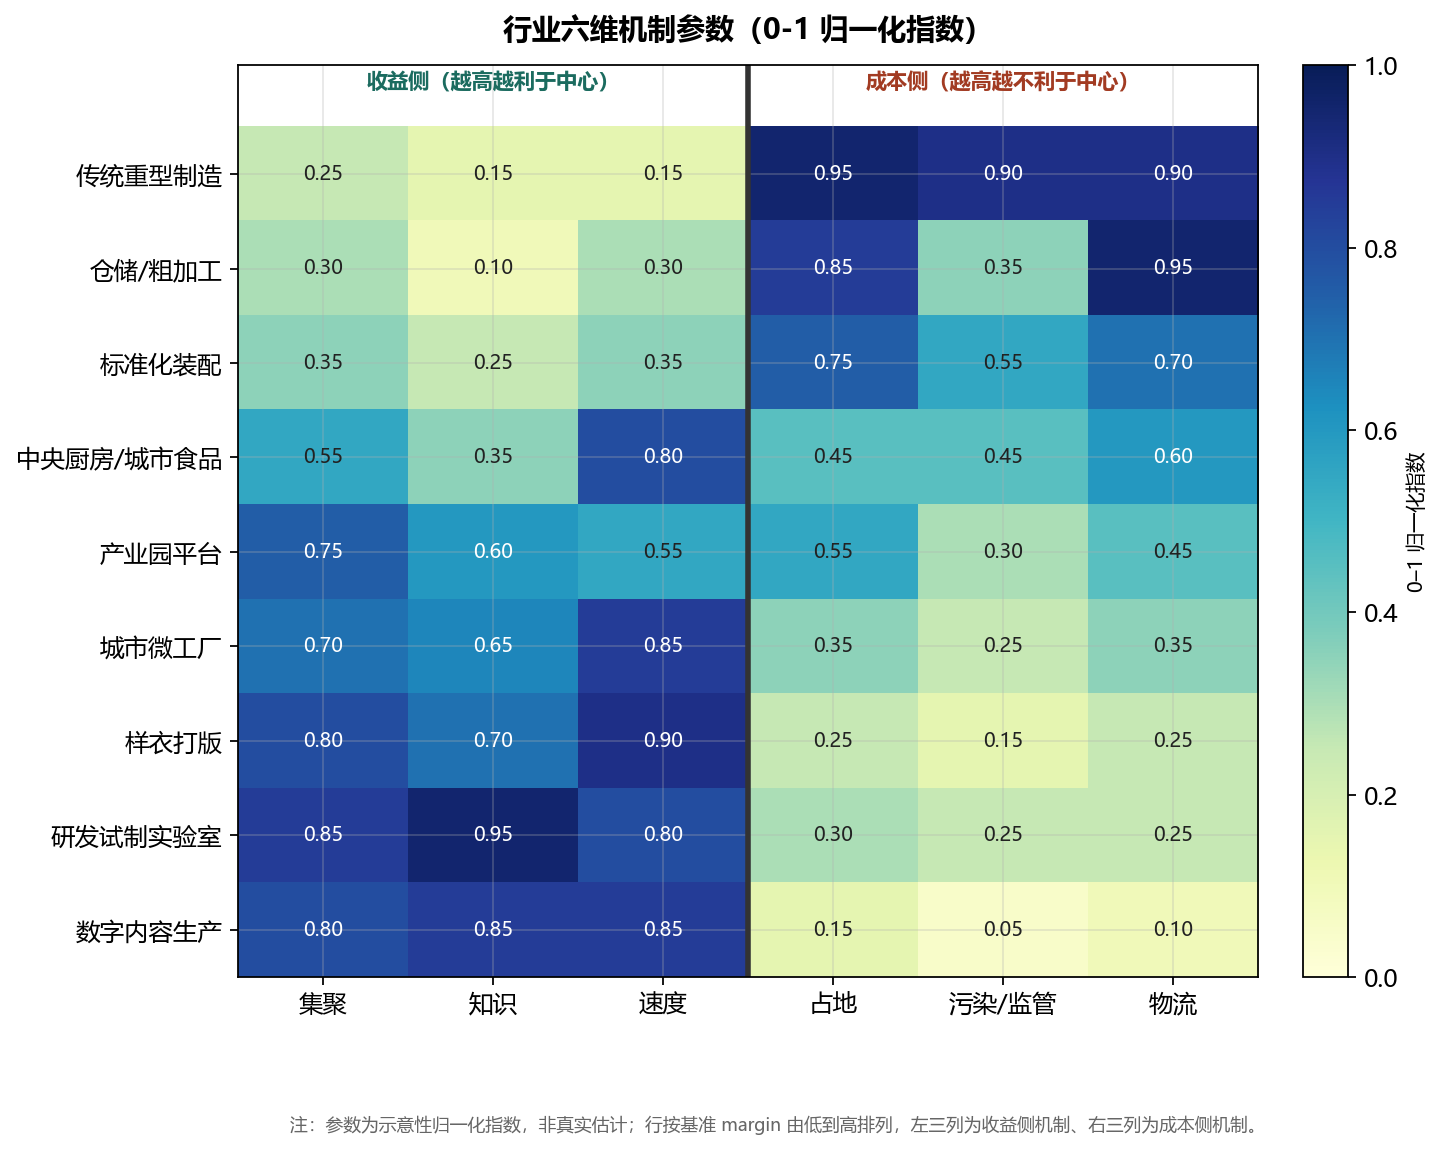
\includegraphics[width=\linewidth]{model_parameter_heatmap.png}
    \caption{行业六维机制参数。左三列为吸引作用，右三列为排斥作用；数值为 0--1 归一化先验参数，按基准情景中心可行性余量由低到高排列。此图用于展示模型中的主观赋值。}
    \label{fig:param_heatmap}
\end{figure}

图~\ref{fig:param_heatmap} 展示了行业参数设定。赋值逻辑是机制性的：数字内容生产天然低占地、低污染、低物流依赖，却高度依赖知识和快速迭代；传统重型制造则相反。研发试制、样衣打版和城市微工厂位于两者之间，但收益侧明显高于传统制造。情景参数也按同一原则设定：中心地租上升情景提高地租权重；低负外部性生产情景降低污染/监管、物流摩擦和一般拥挤的惩罚权重；远程办公情景降低共址集聚收益。

在这些先验参数上，定义一个唯象的线性阈值模型。对生产类型 $i$ 和情景 $s$，下式中的 $\tilde B_{is}$ 和 $\tilde C_{is}$ 分别表示中心收益指数和中心成本指数，二者处在同一描述性标度：
\begin{align}
\tilde B_{is} &= \alpha_s A_i+K_i+V_i,\\
\tilde C_{is} &= r_s L_i+\rho_s P_i+\ell_s G_i+\Gamma_s 
\end{align}
其中 $\alpha_s,r_s,\rho_s,\ell_s$ 表征情景 $s$ 下集聚收益、地租、监管和物流压力的相对权重；$\Gamma_s$ 是同一情景下的一般拥挤成本。这里的拥挤不是指货运物流（已由 $\ell_sG_i$ 刻画），而是表示中心区共同存在的运营阻力，如人员通勤拥挤、空间功能冲突和协调成本。代码中 $\Gamma_s$ 被简化为同一环境下的共同背景项，不随生产类型变化。中心可行性定义为
\begin{equation}
    \marginvar_{is} = \tilde B_{is}-\tilde C_{is}
\end{equation}
若 $\marginvar_{is}>0$，该生产活动在情景 $s$ 下理论上可以存在于中心；若 $\marginvar_{is}\leq0$，则更适合外围。该模型不估计真实利润，只给出一个可审计的比较框架。

\begin{figure}[!t]
    \centering
    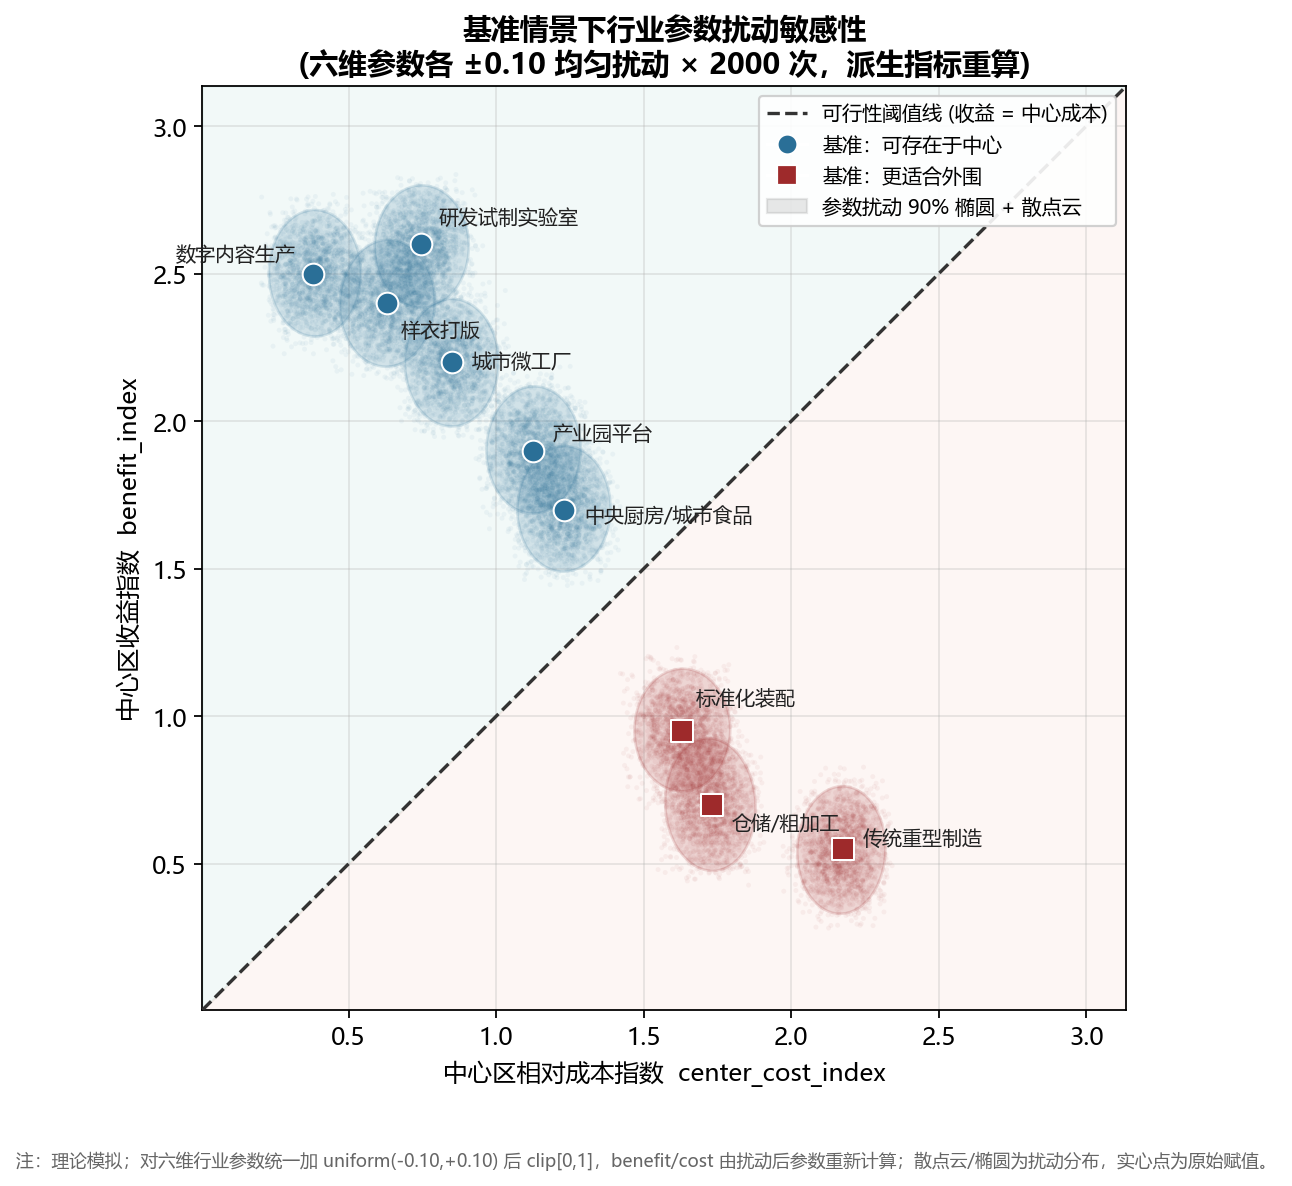
\includegraphics[width=\linewidth]{threshold_phase_diagram_perturbed.png}
    \caption{基准情景下的行业参数扰动相图。实心点为图~\ref{fig:param_heatmap} 中的原始先验赋值；散点云和椭圆来自对六维行业参数统一加入 $\pm0.10$ 均匀扰动并重新计算收益和成本。虚线为收益等于成本的阈值。}
    \label{fig:phase}
\end{figure}

图~\ref{fig:phase} 显示基准情景下的阈值结构和行业参数扰动结果。扰动实验对每个行业的六个先验指标统一加入 $\mathrm{uniform}(-0.10,+0.10)$ 并裁剪到 $[0,1]$，重复 2000 次。数字内容生产、研发试制实验室、样衣打版、城市微工厂、产业园平台和中央厨房/城市食品的始终处于可行阈值以上；传统重型制造、仓储/粗加工和标准化装配的可行概率均为 0.00。也就是说，在该扰动尺度下，核心排序不依赖于某一个精确参数值。

\begin{figure}[!t]
    \centering
    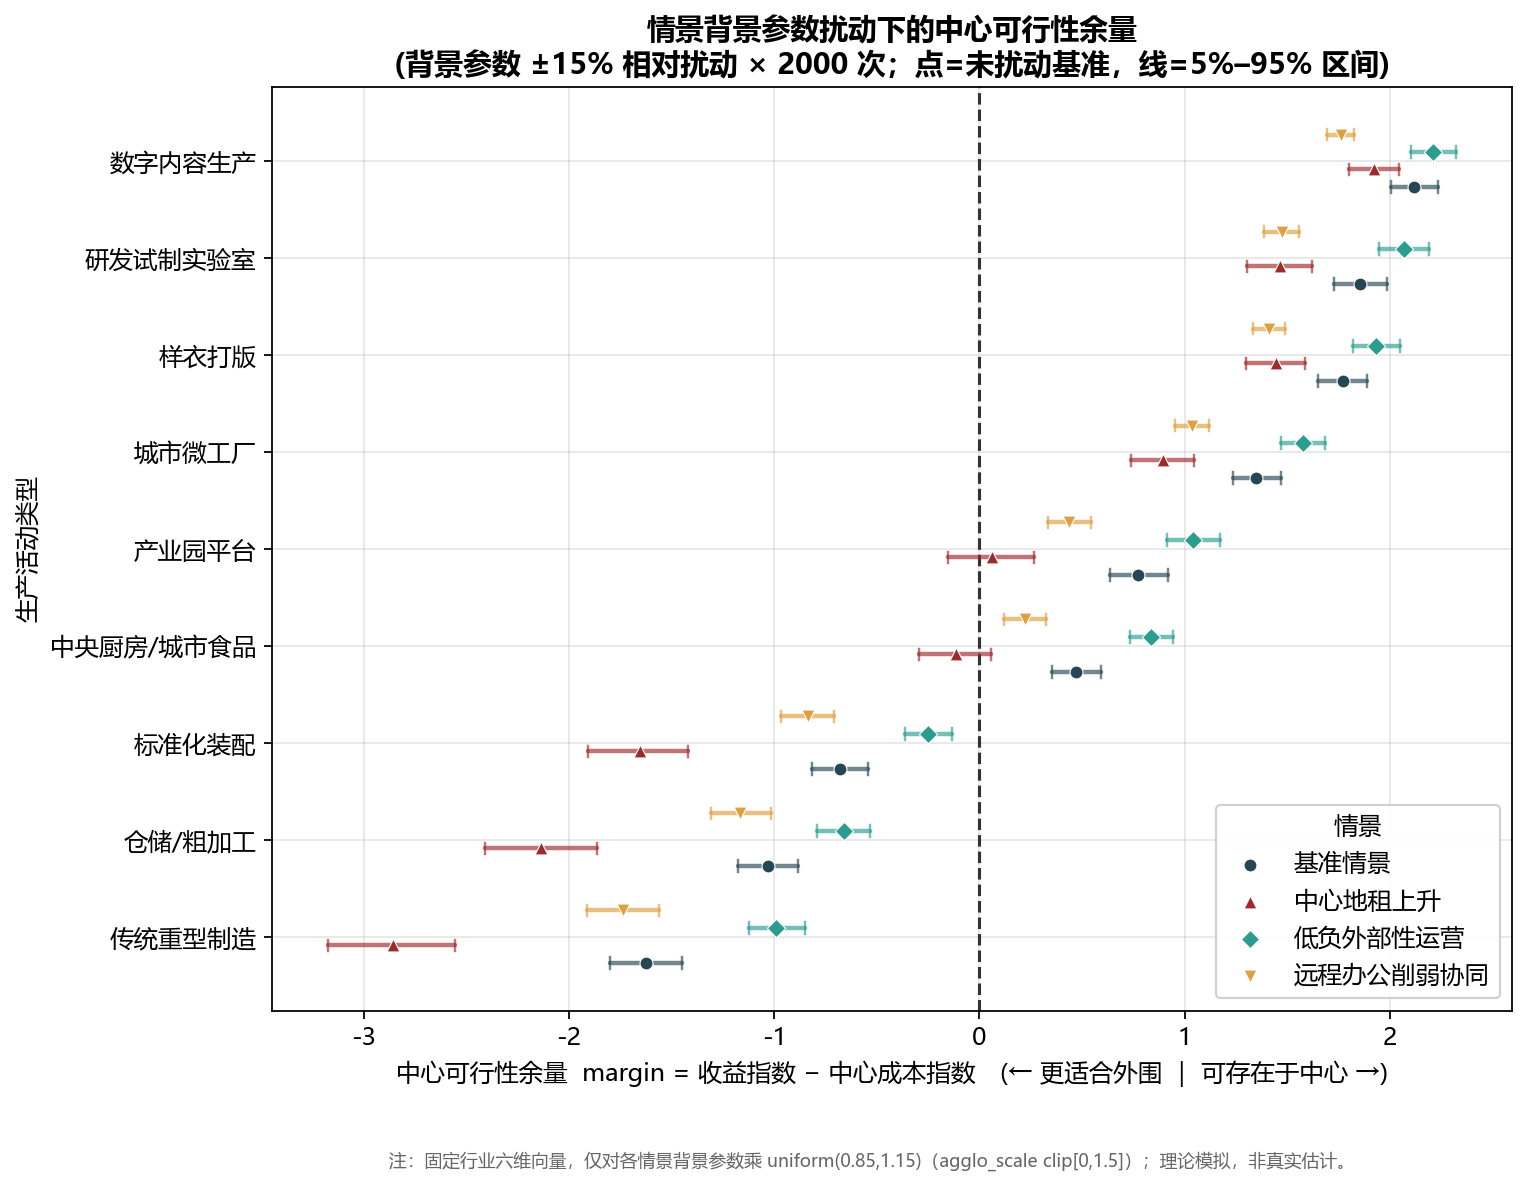
\includegraphics[width=\linewidth]{scenario_comparison_perturbed.png}
    \caption{情景背景参数扰动下的中心可行性余量。行业六维向量保持不变，仅对各情景的背景参数加入 $\pm15\%$ 相对扰动；点为未扰动基准值，线段为 5\%--95\% 区间。}
    \label{fig:scenario}
\end{figure}

图~\ref{fig:scenario} 固定行业六维向量，只扰动情景背景参数。基准、低负外部性生产、远程办公削弱协同三个情景下，六个中心可行类型和三个外围类型均不翻转。中心地租上升情景则显著压缩土地密集型生产，并使中央厨房/城市食品和产业园平台处于临界区域。两端排序仍然稳定：高知识、低外部性活动保持中心可行，传统重型制造、仓储/粗加工和标准化装配保持外围可行。

需要强调的是，随机扰动并不能改变模型使用主观先验参数的事实。另外，此模型存在先天的漏洞：线性标度假定。它默认一个单位的有利因素可以和一个单位的排斥因素相互抵消，而实际经济活动的相对权重大概率是严重非线性且难以量化的。因此，所谓理论模拟只说明在一组可审计、逻辑合理的先验假设下，模型会给出何种排序；真正具有事实约束力的部分，是后文上海 POI 空间分布与这一排序是否相互印证。

\section{上海 POI 描述性证据}

前文的阈值模型只能给出条件判断，为避免结论停留在先验参数内部，必须验证现实城市中的生产活动是否呈现相同的空间分布。为此，本文使用上海生产活动 POI 构造空间样本。POI 是地图数据库中带有名称、类别、地址和经纬度的空间点，适合描述城市设施的空间分布。

样本来自高德地图平台中的生产活动候选点，通过关键词规则自动清洗和分类。输入审计表共 2801 条记录，自动保留 2756 条，过滤消费/零售类误判 44 条，重复剔除 1 条。保留样本包括传统制造 1072 条、城市型生产 476 条、城市食品生产 136 条、产业/园区空间 902 条、难以分类 170 条。这里的``难以分类''并不等于无关样本，我们人工浏览其名称和地址后发现，其中相当一部分仍与高新技术、研发平台有关，只是关键词规则不足以将其纳入某一明确类型。本文保留其独立类别，不把人工印象并入自动分类结果。

尽管近 3000 条 POI 已经能较清楚地展示上海生产活动的空间分布，但本文没有系统比对工商注册企业名录，没有对自动分类结果作抽样人工审查，同时忽略了地图平台选择性收录、关键词采集偏误和因果识别等问题，因此本文采用“描述性证据”这一审慎保守的表述。自动规则会保留一定漏判和误判，但也保证分类结果可复现；只要误差不是系统性地把城市型生产移向中心或把传统制造移向外围，少量误判不太可能解释后文中 8--10 公里的平均距离差。总而言之，POI 分析或许尚不足以证明城市中心因果性地吸引城市型生产，但可以提供一个可复现且规模较大的事实图像，用来检验理论排序是否与现实空间分布大体一致。

\begin{figure}[!t]
    \centering
    {\small\textbf{(a) 单中心口径：距人民广场}}\par
    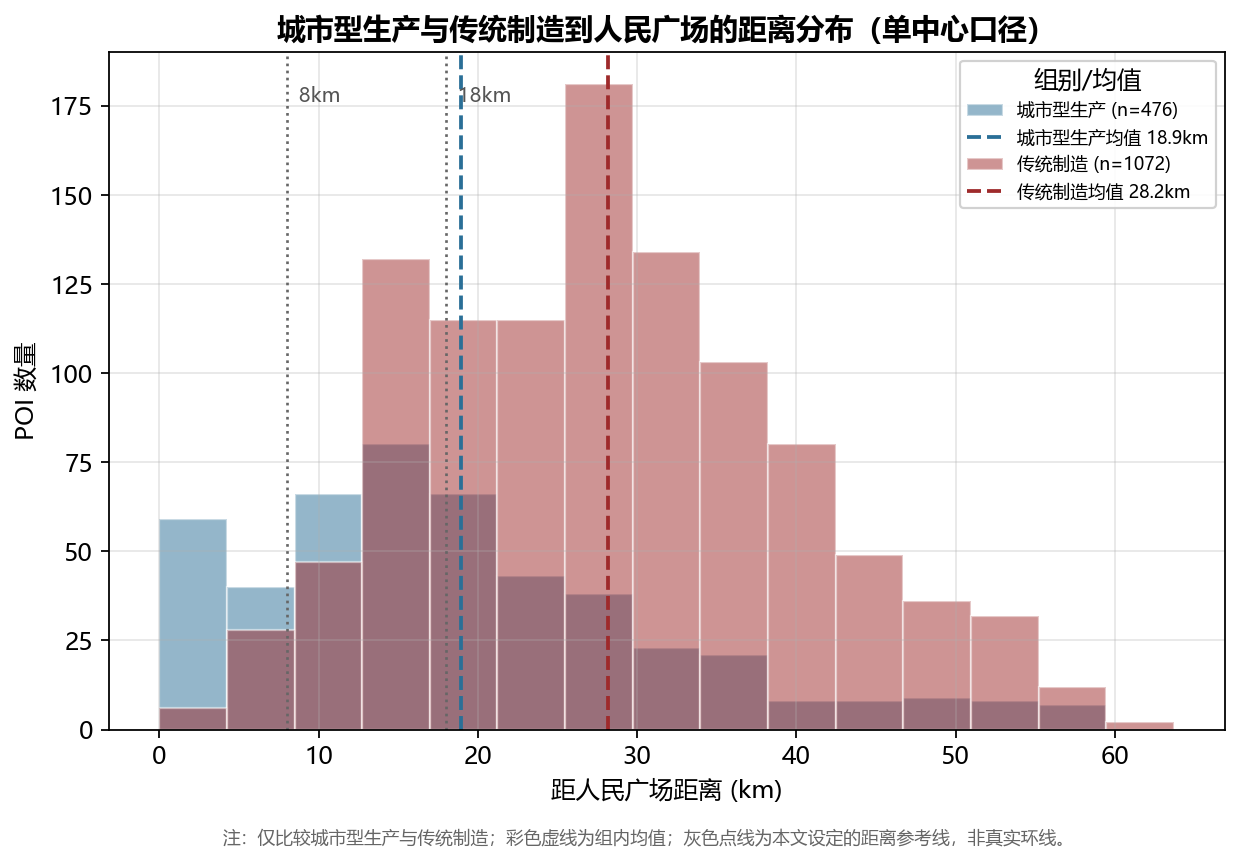
\includegraphics[width=\linewidth]{poi_distance_distribution.png}
    \vspace{0.35em}

    {\small\textbf{(b) 多中心口径：距最近中心/副中心}}\par
    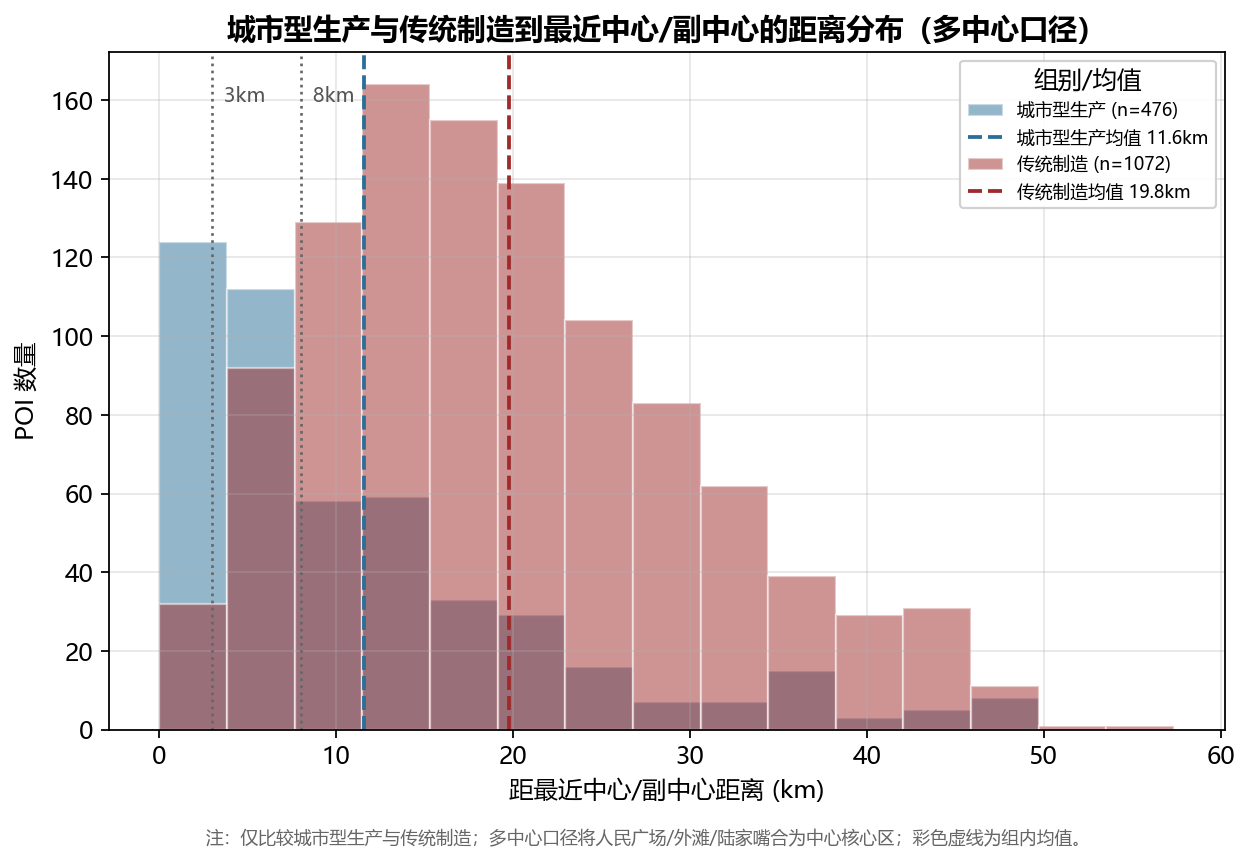
\includegraphics[width=\linewidth]{poi_distance_distribution_polycentric.png}
    \caption{城市型生产与传统制造的中心距离分布对比。上图使用单中心口径，中心点为人民广场；下图使用多中心口径，将人民广场、外滩、陆家嘴合并为中心核心区，并加入徐家汇、五角场、张江、虹桥、前滩等中心/副中心。彩色虚线为组内均值，灰色点线为本文设定的距离参考线。}
    \label{fig:distance_compare}
\end{figure}

\begin{figure}[!t]
    \centering
    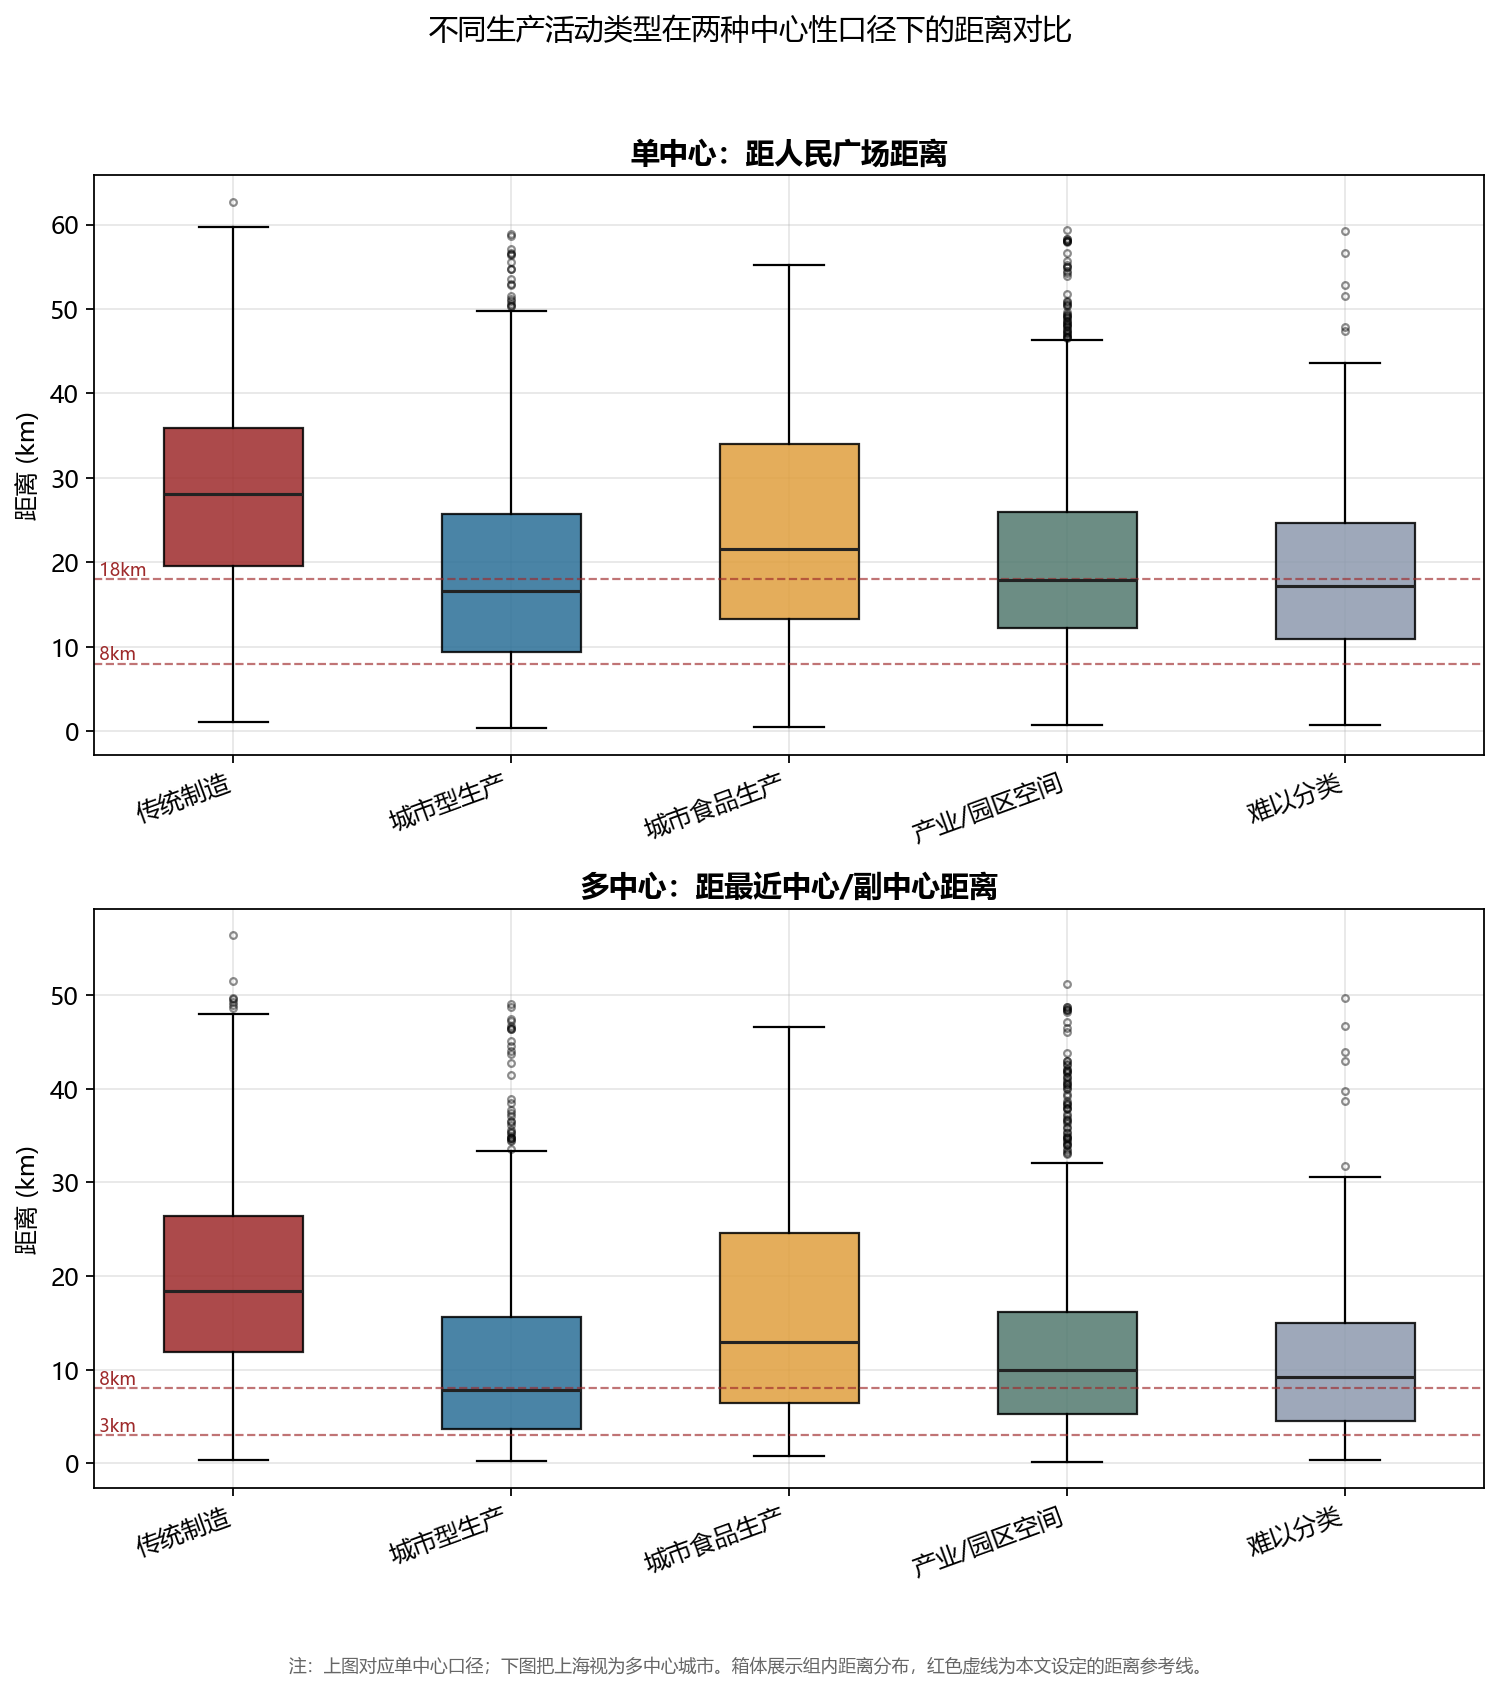
\includegraphics[width=\linewidth]{category_distance_comparison.png}
    \caption{不同生产活动类型在两种中心性口径下的距离箱线图。上图为到人民广场的单中心距离，下图为到最近中心/副中心的多中心距离。两种口径下，传统制造的中位距离均明显高于城市型生产；产业/园区空间更接近城市型生产，说明园区和混合生产空间也可能嵌入中心及副中心附近。}
    \label{fig:box_compare}
\end{figure}

\begin{table}[!b]
\caption{上海生产活动 POI 的类型与中心距离。距离单位为公里。}
\label{tab:summary}
\centering
\scriptsize
\setlength{\tabcolsep}{2.2pt}
\begin{tabular}{@{}lrrrrr@{}}
\toprule
类型 & 样本个数 & 单中心均值 & 单中心中位 & 多中心均值 & 多中心中位\\
\midrule
传统制造 & 1072 & 28.16 & 28.04 & 19.78 & 18.36\\
城市型生产 & 476 & 18.94 & 16.57 & 11.59 & 7.79\\
城市食品生产 & 136 & 24.35 & 21.59 & 16.52 & 12.94\\
产业/园区空间 & 902 & 20.07 & 17.92 & 12.61 & 9.96\\
难以分类 & 170 & 19.16 & 17.24 & 11.55 & 9.22\\
\bottomrule
\end{tabular}
\end{table}

图~\ref{fig:distance_compare} 和表~\ref{tab:summary} 共同给出第一个事实：城市型生产并非只是在平均值上更近于中心，而是整体左偏分布且靠向中心。单中心口径下，城市型生产到人民广场的平均距离为 18.94 公里，中位距离为 16.57 公里；传统制造的对应数值为 28.16 公里和 28.04 公里。图中的 8 公里和 18 公里是本文为便于比较近、中、远距离分布而设定的合理参考线。城市型生产约 19.5\% 位于人民广场 8 公里以内，约 53.4\% 位于 18 公里以内；传统制造只有约 2.3\% 位于 8 公里以内，且约 77.8\% 位于 18 公里以外。这说明差距不是少数极端点制造出来的，而是样本整体呈现出的统计学差异。

上海不是严格单中心城市。现实城市的中心性会受环路、轨道交通、服务设施和多中心结构影响\cite{lec8}。因此，本文进一步把空间距离定义为到最近中心/副中心的距离，其中人民广场、外滩、陆家嘴因空间距离很近而合并为``中心核心区''，并加入徐家汇、五角场、张江、虹桥、前滩等副中心。多中心口径下的 3 公里和 8 公里同样是本文设定的距离参考线，用来判定生产活动是否贴近任一中心或副中心。多中心口径会压缩所有类型的中心距离，但不改变排序：城市型生产到最近中心/副中心的均值和中位数分别为 11.59 公里和 7.79 公里，传统制造则为 19.78 公里和 18.36 公里。若单中心结果只是人民广场定义造成的偏差，引入多中心后差异应明显消失；相反，城市型生产约 51.3\% 位于最近中心 8 公里以内，而传统制造约为 12.3\%。因此，结论在两种统计口径下方向一致，说明这一描述性排序具有一定稳健性。

这些统计结果也直接回扣了图~\ref{fig:phase} 的阈值模型结果。模型中，数字内容生产、研发试制、样衣打版、城市微工厂等类型位于可行阈值线上方；传统重型制造、仓储/粗加工和标准化装配则位于阈值线下方。POI 分布在排序上与模型方向几乎一致，与理论机制相互印证：传统制造依赖大面积厂房、稳定物流和对其负外部性的容忍度，因此，它更适合外围工业园区或低地价地区。城市型生产则处在产品开发、试制、展示、快速交付和定制化环节。它未必需要大规模厂房，却需要靠近设计师、工程师、客户、供应商和专业服务平台。第五讲关于多样化城市和实验室城市的讨论提供了同一逻辑：新产品、新工艺和试错阶段更适合多样化大城市；成熟后的规模化生产再迁往成本更低的专业化城市，在这里上海外围地区可承担后者的职能\cite{lec5}。因此，POI 分布中的距离差异不是孤立的统计现象，而可解释为生产链条不同环节在中心收益和中心成本之间的权衡。

图~\ref{fig:box_compare} 展示了所有类型生产的分布箱线图。除开已经具体讨论过的传统制造与城市型生产，产业/园区空间到人民广场的平均距离为 20.07 公里，到最近中心/副中心的平均距离为 12.61 公里，明显低于传统制造。这反映上海中心/副中心附近存在大量科技园、孵化器和产业平台。它们不是传统意义上的封闭工厂，同时承载研发、试制、展示和小规模生产的混合功能。城市食品生产位于传统制造和城市型生产之间，也符合直觉：中央厨房和食品加工既服务城市消费、需要靠近需求端，又受到物流、环保和占地条件约束。它们处于中间位置同样与图~\ref{fig:phase} 在趋势上符合。

\section{结论}

城市中心可以存在工厂，但这个命题必须改写为更精确的问题：什么类型的生产活动可以存在于城市中心？土地密集、物流密集、污染或安全约束较强的传统制造，在中心区面对高地租、物流和监管压力时通常缺乏竞争力；低土地强度、低负外部性、高知识密度并依赖协同的城市型生产，则可能保留在中心附近。因此，现代城市中心并不是简单地排斥生产，而是在筛选生产的类型。

理论模型和上海 POI 证据给出了相互印证的图像。六维阈值模型把城市中心的吸引作用写成集聚、知识和速度，把排斥作用写成土地强度、污染/监管和物流依赖。尽管模型参数是机制性先验，扰动实验显示，数字内容、研发试制、样衣打版和城市微工厂等类型稳定处于中心可行区域，传统重型制造、仓储/粗加工和标准化装配稳定处于外围区域。上海 2756 条生产活动 POI 的空间分布也几乎呈现同一排序：城市型生产比传统制造更接近人民广场，也更接近最近中心/副中心；产业/园区空间、城市食品生产则介于二者之间。这说明理论中的``中心收益抵消中心成本''并非只停留在参数设定内部，而能在现实城市空间中看到对应的描述性事实。

本文没有尝试证明中心区因果性地吸引城市型生产。因此，更稳妥的结论是：在上海这一多中心城市中，城市型生产相对传统制造更靠近中心，这一事实与课程中关于集聚、竞租、城市规模成本和技术变迁的机制相一致。对城市规划而言，需要认识到生产活动在现代城市中的形态分化已经导致其空间分野。

\begin{thebibliography}{9}

\bibitem{lec2}
吴建峰：《经济与社会》，复旦大学经济学院，课程讲义第 2 讲``为什么出现城市''，2026 年春季学期。

\bibitem{lec4}
吴建峰：《经济与社会》，复旦大学经济学院，课程讲义第 4 讲``城市一定带来经济增长吗？''，2026 年春季学期。

\bibitem{lec5}
吴建峰：《经济与社会》，复旦大学经济学院，课程讲义第 5 讲``城市规模是如何决定的？''，2026 年春季学期。

\bibitem{lec7}
吴建峰：《经济与社会》，复旦大学经济学院，课程讲义第 7 讲``为什么出现摩天大楼？''，2026 年春季学期。

\bibitem{lec8}
吴建峰：《经济与社会》，复旦大学经济学院，课程讲义第 8 讲``城市内部房价如何分布？''，2026 年春季学期。

\bibitem{lec10}
吴建峰：《经济与社会》，复旦大学经济学院，课程讲义第 10 讲``技术革新和城市未来''，2026 年春季学期。

\end{thebibliography}

\section*{AI 使用声明}

本文核心问题、研究思路和主要判断由作者本人提出，包括使用线性阈值模型量化中心区收益与成本、通过扰动实验检验参数稳健性，以及收集上海实际 POI 数据作为描述性证据来印证理论排序。

在写作过程中，作者使用 AI agent 作为辅助工具。AI agent（\texttt{gpt-5.5}）用于总结并串联课程课件，前期初筛可能用于论文的课程知识点；阈值模型中的六维机制变量也在作者与 \texttt{gpt-5.5} 的讨论中逐步提炼完善。代码实现由 AI agent（\texttt{claude-opus-4.8}）辅助完成，并由另一轮 \texttt{claude-opus-4.8} agent 对代码逻辑和结果进行交叉验证。

论文语言由 \texttt{gpt-5.5} 辅助润色，主要包括专业术语使用、论证边界和表述严谨性。例如，本文采用``描述性证据''这一表述，即是采纳 \texttt{gpt-5.5} 的建议：作者原本倾向使用更强的结论表述，但 \texttt{gpt-5.5} 认为若要作更强因果结论，还需要双重差分、事件研究、断点回归、边界设计等识别策略，最终采纳审慎表述。

作者对本文的选题、核心论点、模型设定取向、结果解释和最终文字负责。但需要说明，作者本人是物理学背景，对于 AI agent 在经济学术语、研究范式或方法边界上给出的结果，作者仅能在本课程所学与可理解范围内核对，这是本文需要承认的潜在局限。

\clearpage
\appendix
\section*{Appendix}
\section{模型细节与实验细节}

模型使用归一化无量纲指标描述不同生产活动的属性。收益侧包括集聚收益 $A_i$、知识密度 $K_i$ 和速度价值 $V_i$。成本侧包括土地强度 $L_i$、污染/监管压力 $P_i$、物流依赖 $G_i$，以及情景层面的一般拥挤成本 $\Gamma_s$。权重 $r_s,\rho_s,\ell_s$ 把地租、监管和物流压力映射到同一指数标度；它们不是可直接观测的市场价格。$\Gamma_s$ 对所有生产类型相同，表示中心区共同背景摩擦。不同情景通过改变 $r_s,\rho_s,\ell_s,\Gamma_s$ 或集聚收益缩放系数 $\alpha_s$ 来模拟中心地租上升、低负外部性运营和远程办公削弱协同等情况。所有参数都是机制性先验，不由真实企业利润数据估计。

按 $(\alpha_s,r_s,\rho_s,\ell_s,\Gamma_s)$ 记，四个情景的参数向量分别为：基准情景 $(1.00,0.90,0.70,0.60,0.15)$；中心地租上升 $(1.00,2.20,0.70,0.60,0.15)$；低负外部性运营 $(1.00,0.90,0.20,0.45,0.10)$；远程办公削弱协同 $(0.55,0.90,0.70,0.60,0.15)$。图~\ref{fig:scenario_params} 将同一信息可视化：每个参数下三根柱子表示非基准情景，水平虚线表示该参数的基准值。

\begin{figure}[!b]
    \centering
    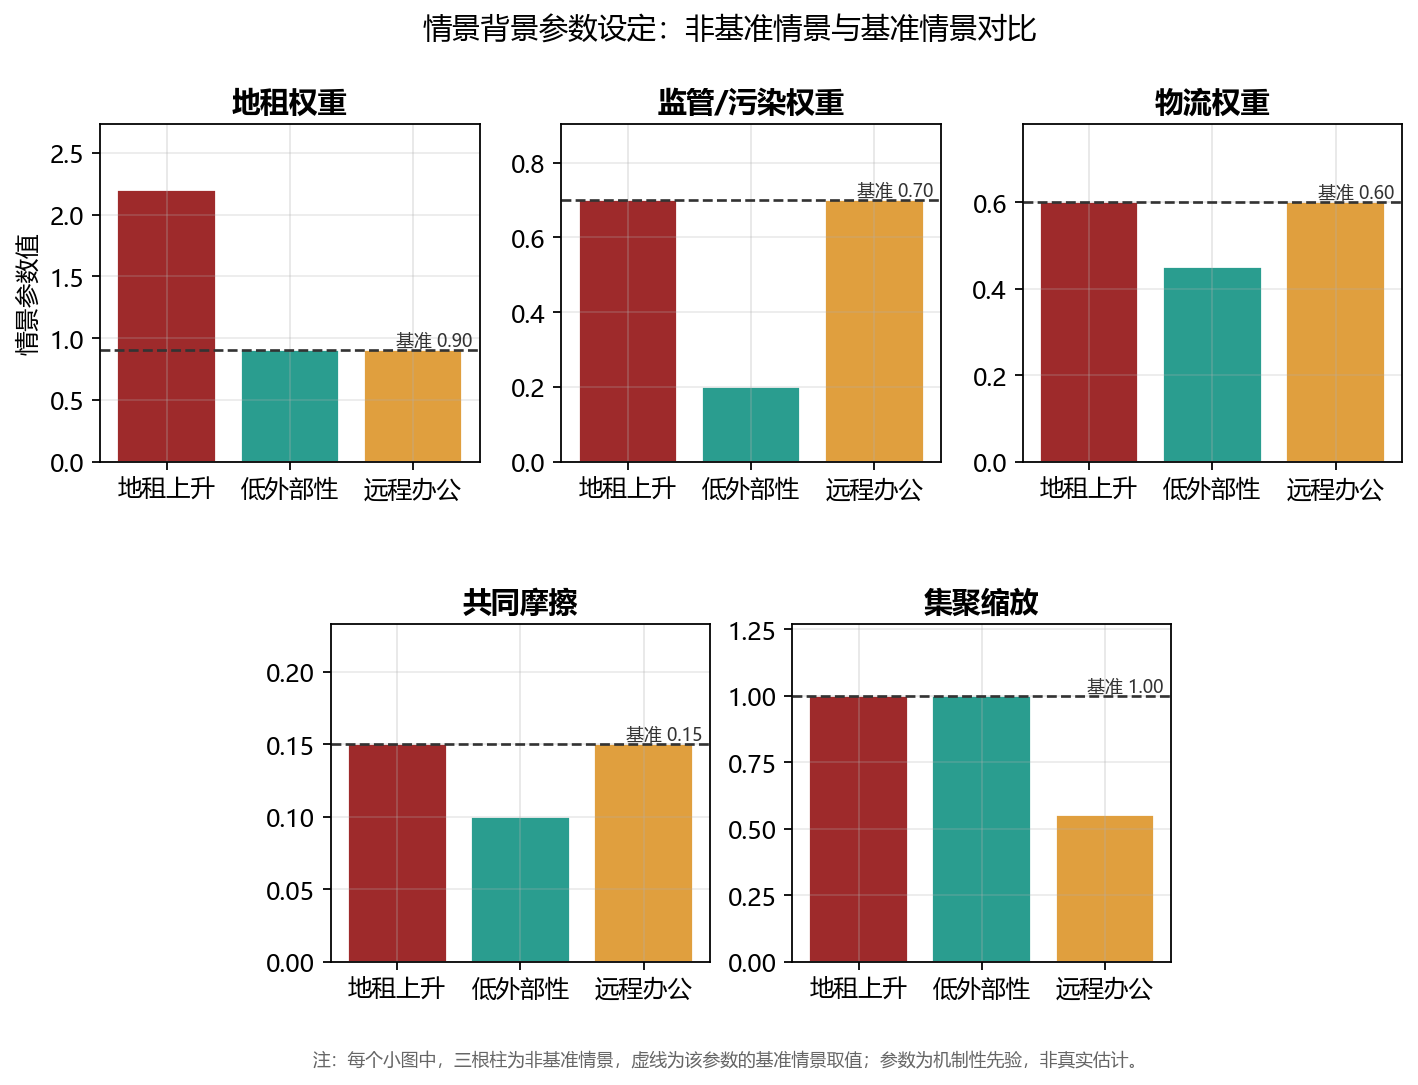
\includegraphics[width=\linewidth]{scenario_parameters.png}
    \caption{情景背景参数设定。每个小图对应一个背景参数，三根柱子为非基准情景，水平虚线为该参数在基准情景中的取值。所有参数均为机制性先验，非真实估计。}
    \label{fig:scenario_params}
\end{figure}

扰动实验有两种模式。第一，在基准情景下，对每个行业的六维参数统一加入 $\mathrm{uniform}(-0.10,+0.10)$，裁剪到 $[0,1]$，重复 2000 次，并用扰动后的六维参数重新计算收益、成本和余量。第二，固定行业六维参数，对每个情景的 $r_s,\rho_s,\ell_s,\Gamma_s,\alpha_s$ 统一乘以 $\mathrm{uniform}(0.85,1.15)$，重复 2000 次。两个扰动都使用同一随机种子和同一规则，不针对单个行业或单个情景作特殊调整。扰动结果只能说明排序对局部误差不敏感，不能消除线性标度假定本身的局限。

该模型与课程中竞租模型的关系是趋势上的，而不是严格推导关系。课程中企业区位支付意愿可写为
\begin{equation}
    \mathrm{Bid\ Rent}=\frac{R-\mathrm{NLC}-T}{S}
\end{equation}
其中 $R$ 是收入，$\mathrm{NLC}$ 是非土地成本，$T$ 是运输或交流成本，$S$ 是占地面积\cite{lec7}。不难看出，竞租能力与收入 $R$ 正相关，与 $\mathrm{NLC}$、$T$ 和 $S$ 负相关。本文的可行性余量 $\marginvar_{is}$ 可以理解为对这种正负相关性的简化表达：收益侧的 $A_i,K_i,V_i$ 对应于中心区可能提高收入、协同效率和迭代速度的因素，因而方向上类似于提高 $R$；成本侧的 $L_i,P_i,G_i$ 以及共同背景摩擦 $\Gamma_s$ 则对应于占地、非土地成本、运输/物流和中心运营阻力，方向上类似于提高 $S$、$\mathrm{NLC}$ 或 $T$。二者在正负相关方向上是一致的，只是具体函数形式不同。本文并不是要提出一个能够经过学界检验的正式结构模型，只是在课程竞租逻辑启发下给出一个描述性的比较框架，便于组织机制讨论和数值模拟。

\section{POI 采集、分类与空间变量}

POI 采集使用高德 Web 服务搜索接口。

\begin{figure*}[!t]
    \centering
    \begin{minipage}[t]{0.42\textwidth}
        \centering
        {\small\textbf{(a) POI 空间分布}}\par
        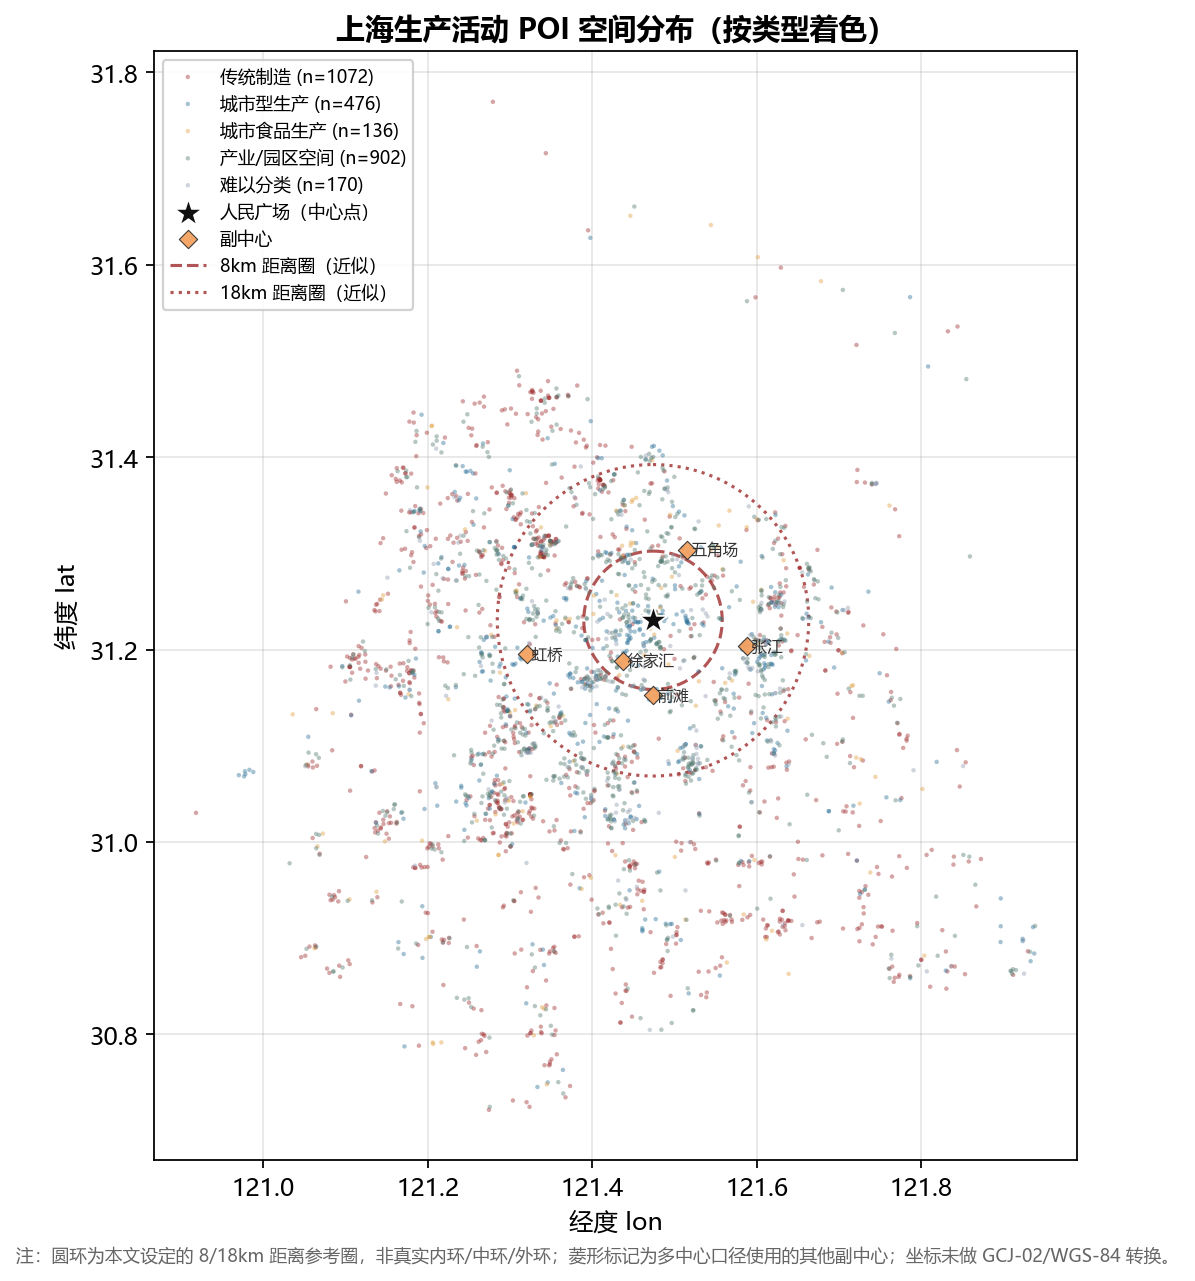
\includegraphics[width=\linewidth,height=0.45\textheight,keepaspectratio]{poi_scatter_map.png}
    \end{minipage}\hfill
    \begin{minipage}[t]{0.55\textwidth}
        \centering
        {\small\textbf{(b) 单中心距离分组：距人民广场}}\par
        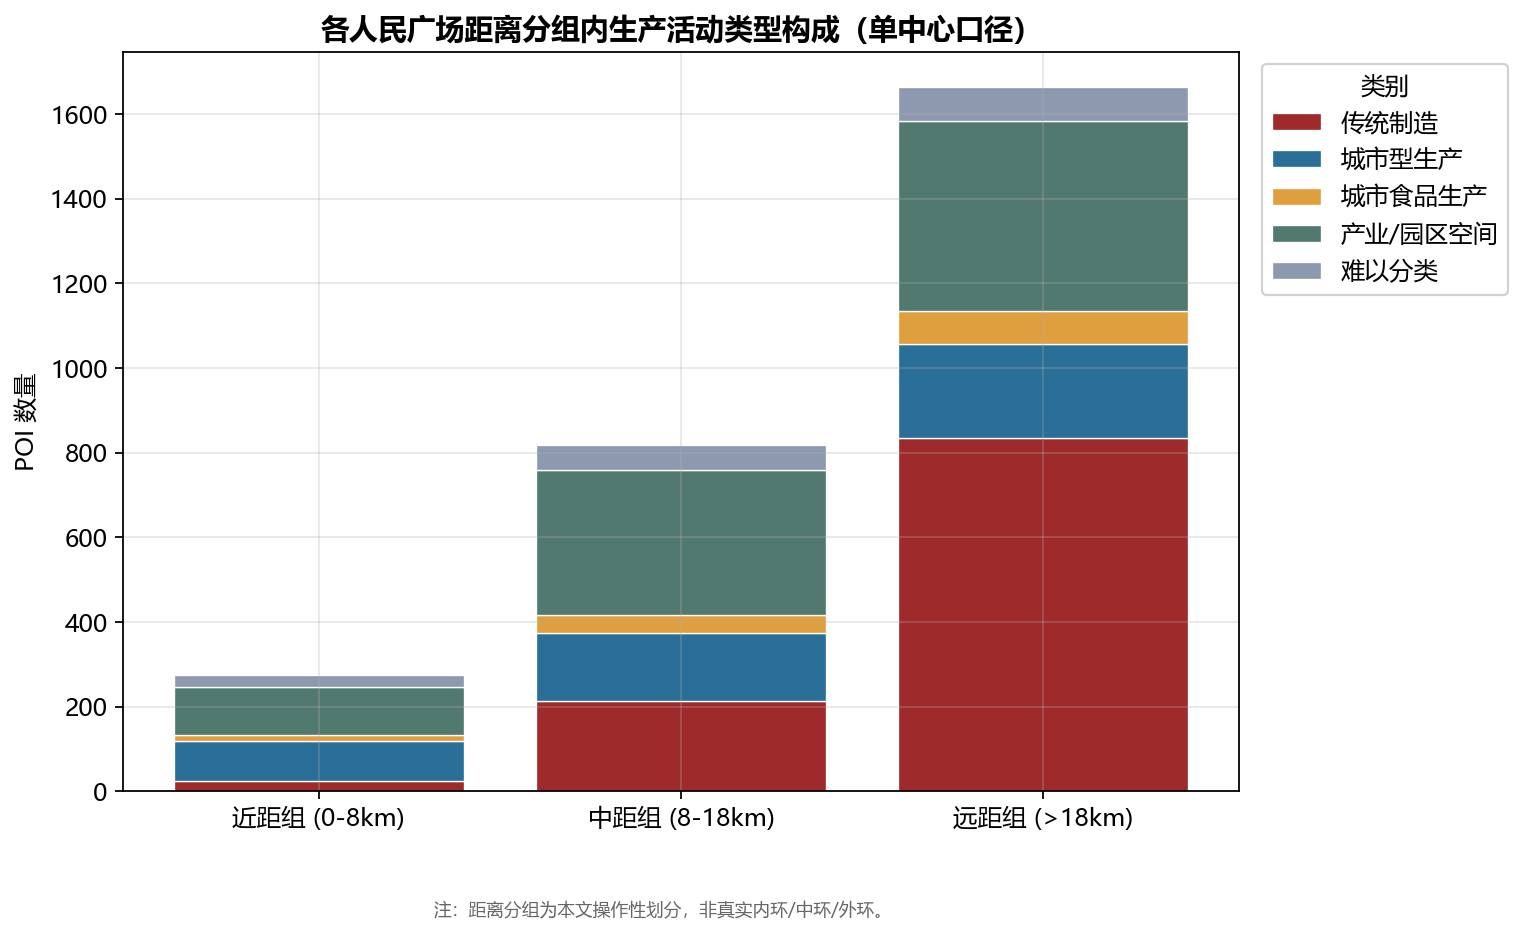
\includegraphics[width=\linewidth,height=0.205\textheight,keepaspectratio]{category_by_zone.png}
        \vspace{0.35em}

        {\small\textbf{(c) 多中心距离分组：距最近中心/副中心}}\par
        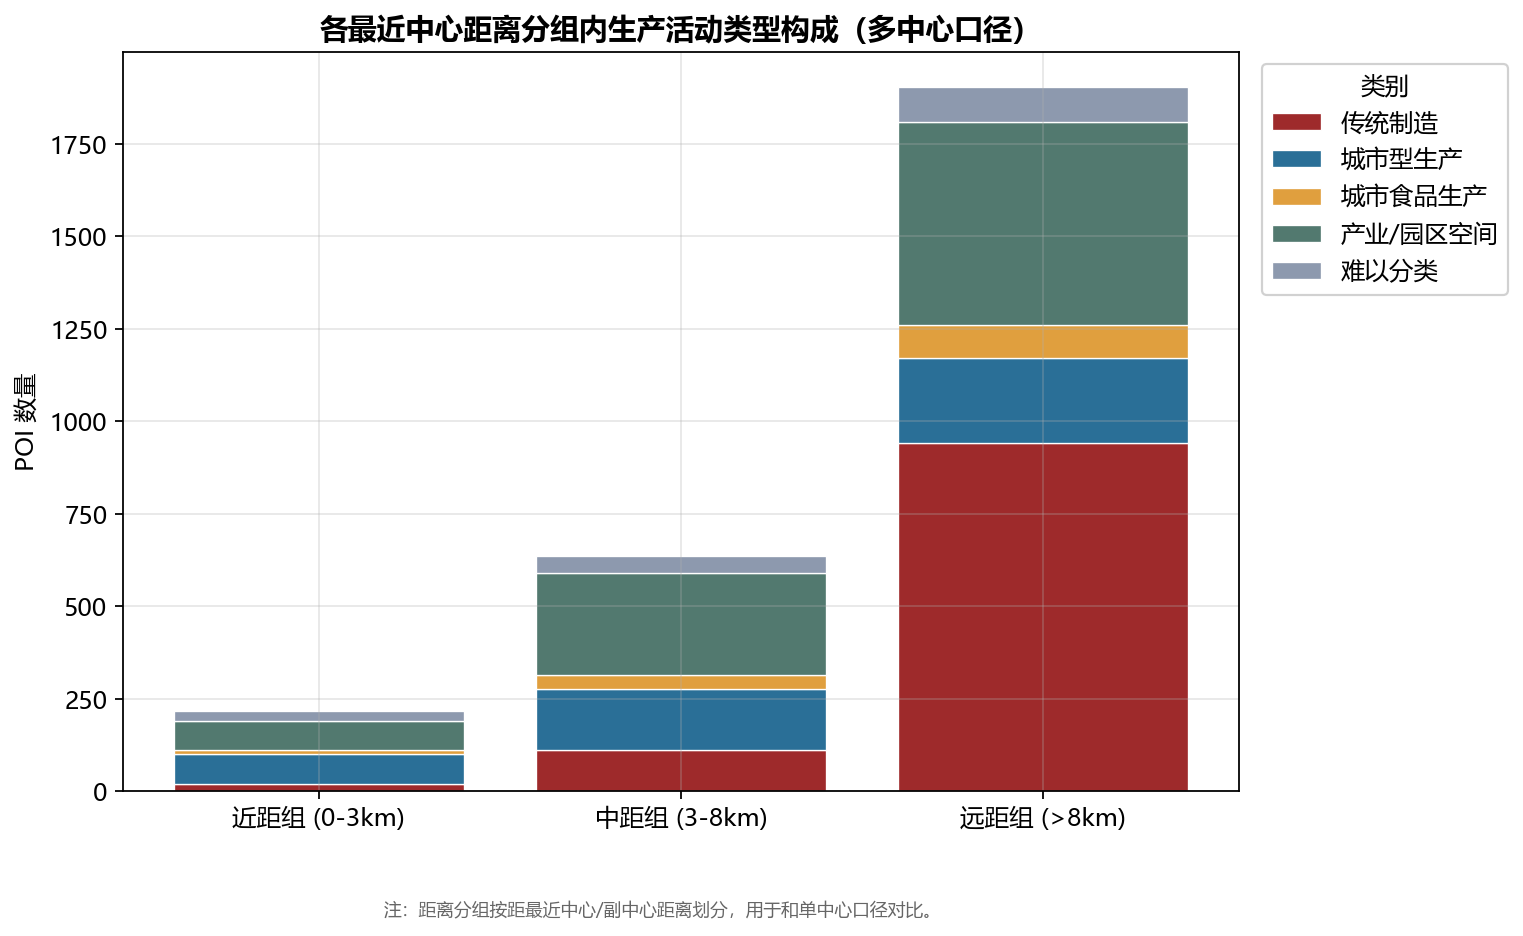
\includegraphics[width=\linewidth,height=0.205\textheight,keepaspectratio]{category_by_nearest_center_zone.png}
    \end{minipage}
    \caption{上海生产活动 POI 的补充空间图。左图展示 POI 样本在上海空间上的覆盖情况；圆环为距人民广场的距离参考圈，不对应真实环线或标准边界。右侧两图展示不同中心性口径下距离分组内的生产活动类型构成；距离组是本文的操作性划分，不是标准城市边界。}
    \label{fig:scatter}
    \label{fig:zone_compare}
\end{figure*}

检索关键词完整列表为：``工厂''、``制造''、``加工''、``机械厂''、``电子厂''、``印刷厂''、``包装厂''、``样衣''、``打版''、``服装设计''、``研发中心''、``实验室''、``试制''、``3D打印''、``中央厨房''、``烘焙工厂''、``食品加工''、``产业园''、``工业园''、``科技园''、``创意园''、``孵化器''。

检索行政区完整列表为：黄浦区、徐汇区、长宁区、静安区、普陀区、虹口区、杨浦区、浦东新区、闵行区、宝山区、嘉定区、松江区、青浦区、奉贤区、金山区、崇明区。默认城市为上海。

采集结果按高德 \texttt{id} 去重，若无 \texttt{id}，则按 \texttt{name+location} 去重；默认与已有输出增量合并，原始表按 \texttt{id, name, location} 去重，中间表按 \texttt{name, address, lon, lat} 去重。脚本将返回结果统一为 \texttt{name, address, lon, lat, raw\_keyword, raw\_type, source} 字段；若原始字段中只有 \texttt{location=lon,lat}，则先解析为经纬度。

清洗规则如下：

第一，坐标必须落入上海经纬区域 $$119.0\leq lon\leq123.0 \text{且} 30.0\leq lat\leq32.5$$

第二，在坐标有效记录中去重：先按 \texttt{name+address} 去重，再按 \texttt{name+lon/lat} 去重，其中经纬度保留到小数点后四位，约等于十米量级；

第三，在保留记录中应用误判过滤和分类规则，所有输入行及其状态均写入 \texttt{poi\_classification\_audit.csv} 供人工审阅。

误判过滤规则为：

若文本命中``中央厨房''、``烘焙工厂''、``食品加工''、``食品厂''、``净菜''、``预制菜''、``中央工厂''等生产性覆盖关键词，则不作为消费误判过滤。

否则若命中``工厂店''、``工厂直销店''、``工厂风''、``工厂主题''、``折扣店''、``奥特莱斯''、``outlets''、``专卖店''、``体验店''、``旗舰店''、``餐厅''、``餐饮''、``咖啡''、``酒吧''、``奶茶''、``火锅''、``烧烤''、``小吃''、``面馆''、``甜品''、``酒店''、``宾馆''、``KTV''、``网咖''、``美发''、``理发''、``健身''、``超市''、``便利店''、``菜场''、``菜市场''，则标记为消费/零售误判并过滤。

分类顺序是有意设定的，因为先后顺序会影响包含泛化词的名称。

第一，若命中``创意工厂''、``梦工厂''、``梦想工厂''，直接归为难以分类。

第二，若命中食品生产关键词``中央厨房''、``烘焙工厂''、``食品加工''、``食品厂''、``净菜''、``预制菜''、``中央工厂''、``冷链''、``糕点厂''、``乳品''、``肉类加工''、``水产加工''、``饮料厂''，归为城市食品生产。

第三，若命中城市型生产关键词``样衣''、``打版''、``打样''、``服装设计''、``设计打样''、``设计制造''、``3d打印''、``3D打印''、``增材制造''、``快速成型''、``原型''、``手板''、``研发试制''、``试制''、``中试''、``小批量''、``定制生产''、``研发中心''、``研发实验室''、``试制实验室''、``工程实验室''、``设计中心''，归为城市型生产。

第四，若仅命中``实验室''，且同时含有``研发''、``试制''、``中试''、``工程''、``材料''、``生物医药''等生产/研发线索，则归为城市型生产；否则归为难以分类。

第五，若命中产业/园区关键词``产业园''、``工业园''、``科技园''、``创意园''、``孵化器''、``软件园''、``文创园''、``众创空间''、``加速器''、``科技城''、``产业基地''、``创业园''、``园区''，归为产业/园区空间。

第六，若命中传统制造关键词``机械厂''、``化工厂''、``化工''、``金属制品''、``金属''、``印刷厂''、``印刷''、``包装厂''、``包装''、``电子厂''、``电子装配''、``装配厂''、``铸造''、``锻造''、``纺织厂''、``钢铁''、``水泥''、``塑料厂''、``橡胶''、``五金''、``机床''、``制造厂''、``加工厂''、``制造''、``加工''、``工厂''，归为传统制造。

若上述规则均未命中，则归为难以分类。

空间变量规则如下。单中心距离以人民广场为中心点，并用 haversine 距离计算。为了描述距离分布，本文把单中心距离人为分为 0--8 公里、8--18 公里和 18 公里以上三组。多中心口径将人民广场、外滩、陆家嘴合并为中心核心区 $(121.4878,31.2364)$，并加入徐家汇 $(121.4368,31.1885)$、五角场 $(121.5147,31.3039)$、张江 $(121.5876,31.2034)$、虹桥 $(121.3205,31.1949)$ 和前滩 $(121.4732,31.1524)$；每个 POI 的多中心距离是其到最近中心/副中心的距离。多中心距离人为分为 0--3 公里、3--8 公里和 8 公里以上三组。这些分组只用于描述和作图，不是真实内环/中环/外环，也不是规划或经济理论中的标准边界。

原始数据和交互页面发布于 GitHub Pages：\href{\DataPageUrl}{\DataPageUrl}。其中原始 POI 数据为 \href{\RawPoiDataUrl}{amap\_poi\_raw.csv}，完整分类审计表为 \href{\AuditDataUrl}{poi\_classification\_audit.csv}。

\end{document}
